\chapter{Antecedentes}
\label{chapter:chapter02}

Existen distintos trabajos que contemplan una comparación entre estrategias mono-objetivo y multiobjetivo para distintos campos de la industria, por ejemplo Jiao, Zeng\cite{Jiao2017DynamicME} entre otros hacen uso de distintas estrategias para convertir un problema mono-objetivo en uno multiobjetivo dinámico en el cual aplican un algoritmo evolutivo multiobjetivo con una mejora en los resultados comparándola con las soluciones existentes. Otro tema muy recurrente en los cuales se comparan su desempeño es en el diseño de antenas para mejorar la recepción telefónica, como es el caso del trabajo de Rahmat-Samil y Nanbo Jin.\cite{Jin2007-qu} 

Por último Battiti y Passerini\cite{Battiti2010-xo} hablan sobre el uso de algoritmos genéticos que se adaptan al tomador de decisiones, esto resulta relevante porque en la plataforma final el usuario propiamente no tiene una decisión real sobre a qué grupo terminará siendo asignado sino que esto se pretende realizar de manera automática, Battiti menciona algunas de las estrategias posibles para que pueda adaptarse el comportamiento de un tomador de decisiones y además discute algunas de las limitaciones que un sistema de este tipo presentaría de acuerdo con sus preferencias.\cite{Wang2010-zh} \\

\section{Optimización Mono-Objetivo}
La optimización mono-objetivo o optimización global es un tipo de problemas que consiste en encontrar el mínimo o el máximo global de una función, ya que en una función no lineal pueden haber mínimos locales, pero un mínimo global es más difícil de encontrar, también es importante tomar en cuenta que se considera un dominio de soluciones y otras limitantes, por lo que en general la solución más obvia suele ser realizar una búsqueda exhaustiva probando cada uno de los valores del dominio, sin embargo esta estrategia puede llegar a ser bastante ineficiente. En los problemas no lineales una función puede contener un número muy largo de máximos y mínimos, a estos se les denominan mínimos o máximos locales, y para encontrarlos basta con usar un método local de optimización clásico.[1], [7], [8] \\

Los algoritmos para encontrar un mínimo global comprenden métodos exactos y heurísticos. Dentro de los algoritmos exactos existen La búsqueda exhaustiva, búsquedas bayesianas, aproximaciones sucesivas y algunos algoritmos estocásticos como el muestreo de Monte-Carlo en el cual una simulación aleatoria es usada para encontrar una solución aproximada, Tuneleo estocástico, etc.[7] \\

\section{Optimización multiobjetivo}

La optimización multiobjetivo es un área del análisis de decisión de múltiples criterios que se encuentra directamente relacionada con los problemas de optimización matemática, que involucra más de una función objetivo para que sea optimizada simultáneamente. [4] \\

Estas soluciones pueden tener distintos criterios o características para ser consideradas opciones óptimas, por lo que se les denominan soluciones de pareto. Una solución Óptima de Pareto se define como una solución cuyas funciones objetivo pueden ser mejoradas sin degradar el resto de las funciones. Se refiere a una solución no dominada en el espacio de criterio del problema. \\

Para los problemas de optimización multiobjetivo no triviales no existe una solución ideal óptima, sino que existen distintas soluciones que optimizan simultáneamente cada objetivo, en cuyo caso se dice que las funciones son contradictorias y existe un número de soluciones óptimas de Pareto. Todas las soluciones que son óptimas por Pareto se dice que son igualmente buenas para los objetivos que se hayan determinado.[4], [5] \\

Usualmente la idea de resolver un problema multiobjetivo es entendido como ayudar a un tomador de decisiones a considerar múltiples objetivos simultáneamente y encontrar una solución óptima de pareto que a su discreción sea más adecuada. Por lo que el método para encontrar la solución requiere de un involucramiento del tomador de decisiones y es influenciado fuertemente por sus preferencias. Usualmente en este tipo de problemas solo se toma en cuenta un sólo tomador de decisiones pero también existe la posibilidad de múltiples tomadores de decisiones. [9]

\section{Algoritmos evolutivos}

Los algoritmos evolutivos forman parte de la computación evolutiva, son algoritmos basados en una población meta-heurísticos para resolver problemas de optimización. Un algoritmo evolutivo usa mecanismos inspirados en la evolución biológica como pueden ser la reproducción, mutación, recombinación y selección, las soluciones candidatas a la optimización forman parte de una población y una función de ajuste determina la calidad de cada una de estas soluciones. Este ajuste toma parte después de distintas iteraciones o generaciones en las que se busca acercarse lo más posible a la función objetivo.[10] \\

Usualmente este tipo de algoritmos tiene un buen desempeño, ya que no se encuentran influenciados directamente por una función de ajuste, la única que interacción que tienen con ésta resulta ser la de un filtro para definir las poblaciones subsecuentes. El uso de estos algoritmos para el modelado de la evolución biológica se limita únicamente a la exploración de micro-evolución o la determinación de sistemas de procesos celulares, por lo que suelen ser más comúnmente usados en problemas donde la complejidad computacional resulta un factor prohibitivo. De hecho la complejidad computacional se deriva directamente de la función de ajuste. La aproximación a esta función es una de las soluciones que supera esta dificultad. [11] \\

En este proceso hay dos fuerzas fundamentales que forman la base de los sistemas evolutivos: \\
\begin{itemize}
\item Los operadores de variación (que son de recombinación y mutación) crean la diversidad necesaria y por lo tanto facilitan la posibilidad de encontrar nuevas soluciones.
\item La selección actúa como una fuerza que empuja la calidad.
\end{itemize}

Los algoritmos evolutivos poseen un número de características que pueden ayudar a posicionarse dentro de las familias de métodos de generación y prueba:

\begin{itemize}
\item Son basados en poblaciones, esto significa que procesan una cantidad variable de soluciones candidatas de forma simultánea.
\item Usualmente usan una recombinación para mezclar la información de más candidatos en soluciones nuevas.
\item Estos algoritmos son estocásticos.
\end{itemize}


Un algoritmo evolutivo generalmente cuenta con los siguientes componentes:

\begin{itemize}
\item Representación (definición de las soluciones)
\item Función de evaluación (o función de ajuste)
\item Población
\item Selección de padres
\item Operaciones de variación, recombinación y mutación
\item Mecanismo de selección de sobrevivientes 
\end{itemize}


Cada uno de estos componente se deben de ser especificados para definir un algoritmo en particular, por lo tanto la inicialización del algoritmo tanto como la condición de terminación deben de ser definidas también.[11]

A continuación se describen los pasos que lleva a cabo un algoritmo evolutivo comúnmente:

\begin{enumerate}
\item \textbf{Inicialización}: Se generan distintas soluciones de forma aleatoria
\item \textbf{Evaluación}: Cada una de las soluciones pasa a ser evaluada por la función de ajuste y se determina que tanto se acerca a su valor óptimo
\item \textbf{Terminación}: Se determina si se alcanzó el objetivo con alguno de los candidatos o si se sobrepasó el número de generaciones límite que se estableció previamente.
\item \textbf{Selección}: Se selecciona las soluciones que "sobreviven" y pasan a la siguiente generación
\item \textbf{Variación}: este paso puede darse por medio de del paso de "cromosomas" o características de las soluciones que sobrevivieron en el paso anterior para combinarse entre sí y dar nuevas soluciones "hijas", el otro método es la mutación, donde una o varias de las características se modifica de manera aleatoria para introducir un nuevo valor a la población
\end{enumerate}


Este ciclo se repite dando paso cada vez a nuevas generaciones que cada vez se ajustan más a la función de evaluación hasta que se alcance el resultado deseado determinado por el paso de Terminación.[10] \\

\section{AMI Meeting Corpus}

Ya que no hay ningún paper que diga que función usar para esto se le hizo un análisis de datos al AMI meeting corpus para ver qué relación había entre el número de silencios y la homogeniedad de las participaciones de acuerdo con los functional roles de Benne y Sheats, y pues resulta que si hay una correlación con respecto al porcentaje de participaciones por lo que se usó esta medida para tratar de predecir la interacción del grupo, considerando que esta participación debe ser homogénea entre ellos por lo que es el inverso a la suma de las participaciones.
[...]
Esta ha sido usada en varios trabajos como para predecir estilos de participación como es el caso de Vinciarelli\cite{VinciarelliUnderstandingCorpus} quien usa esta base de datos para identificar los roles funcionales de Benne y Sheats\cite{benne_sheats}. 

\section{Roles funcionales de Benne and Sheats }
Los roles funcionales de Benne y Sheats son una herramienta que ayuda a definir que tipo de reacción tiene una persona al momento de entablar una conversación[ref]. Los roles en los que estamos interesados específicamente se conocen como los \textbf{Roles de mantenimiento} o sociales que están basados en el trabajo de Biddle [ref] sobre la teoría de los roles, ya que el resto de las definiciones de roles que son los enfocados a tareas y disfuncionales no proporcionan información relevante para la investigación. Estos roles en específico se definen a continuación:

\begin{itemize}\break

\item \textbf{Atacante}: Es aquella persona que invalida los comentarios de otros y "ataca" al resto de los miembros del grupo.
\item \textbf{Protagonista}: es aquella persona que inicia las conversaciones, asume un rol de autoridad. En este caso es un rol muy valioso para nuestra investigación.
\item \textbf{Seguidor (Supporter)}: esta persona presenta una actitud cooperativa, pone atención a la platica, acepta las propuestas y ofrece soporte técnico.
\item \textbf{Gatekeeper}: es una persona que desempeña el rol de moderador, revisando que cada persona tenga su oportunidad de participar de forma similar.
\item \textbf{Neutral}: Es similar al rol de seguidor, sólo que en lugar de participar de forma activa, acepta los comentarios de forma pasiva.
\end{itemize}

Cabe destacar que una persona puede representar distintos tipos de roles en una misma conversación, aunque generalmente se le clasifica dependiendo de cual fue su rol más prominente, lo cual será usado como ventaja, ya que en la base de datos de \textbf{AMI meeting corpus} las etiquetas de los roles están dadas para cada participación y no necesariamente para cada persona, por lo que nos es posible determinar que porcentaje represento cada rol del tiempo total de lo que duro la conversación.

\section{Facebook Ad Platform} 
La red social conocida como Facebook es útil hoy en día para mantener el contacto entre amigos y conocidos, sin embargo también es una útil herramienta de mercadotecnia para dar a los usuarios que pertenecen a un cierto mercado anuncios enfocados a cada uno de ellos acorde a sus preferencias, comportamientos y ubicación, esto de hecho sigue una metodología de la mercadotecnia conocida como Demografía, comportamientos e  intereses[ref]. Por lo que para esta investigación respecta solo nos interesa la cuestión de los intereses. 

Estos intereses están determinados por la clasificación de las paginas o grupos a las que el usuario sigue, sin embargo cuenta con una clasificación más general a manera de una ontología que Facebook ha estado construyendo a lo largo de los años usando distintas técnicas de clustering para que pueda tener una categorización más general de los distintos tipos de intereses de cada uno de los usuarios.

Además Facebook permite que a través de una plataforma conocida como Facbook Ad platform en la cual los negocios pueden hacer uso de ella para publicar distintos tipos de anuncios dirigidos a un tipo de mercado de acuerdo con los intereses o comportamientos que cada uno describe, e. esta plataforma es publica y puede hacerse uso de ella para determinar un costo aproximado al momento de preparar campañas de mercadotecnia. Sin embargo para esta investigación se usa con otro tipo de propósito, en este caso se usa para determinar el tamaño de población para cada uno de los intereses que se describe como será mencionado en las secciones [ref1] y [ref2]. 

También esta plataforma puede ser usada al mismo tiempo para generar la distribución de los datos ya que esta directamente ligada con la ontología y puede ser consultada para medir las distancias entre un interés y otro. Parte de la ontología puede ser vista en la Fig [ref]

\begin{figure}
    \centering
    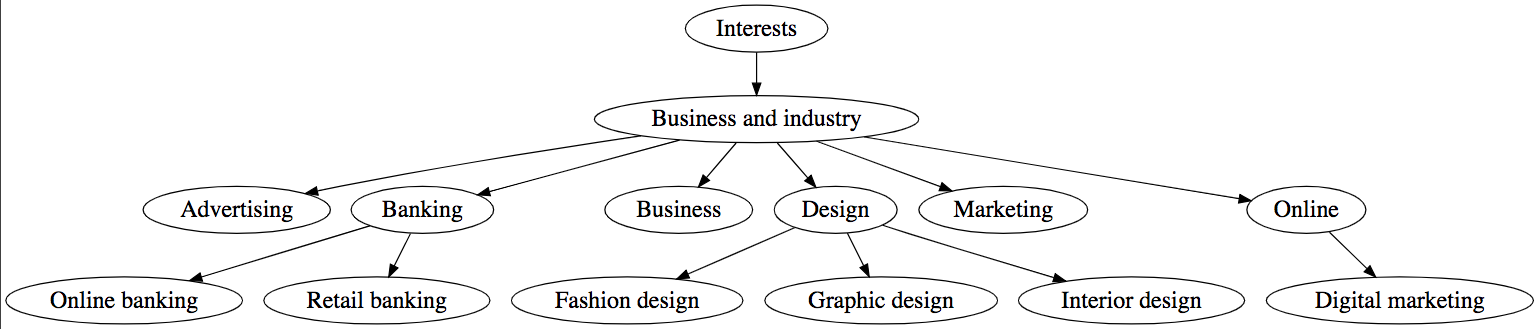
\includegraphics[width=150mm]{ontology.png}
    \caption{Caption}
    \label{fig:my_label}
\end{figure}

La ontología que ha creado Facebook se determina con un arbol de 8 intereses generales y 314 específicos cada uno clasificado según la relación a un interés general, esto nos permite buscar intereses específicos en común, por ejemplo si una persona le gustan los programas de televisión podemos asumir también que le gustan los reality shows o los programas de concursos etc, de esta forma otra persona que tenga un gusto de por ejemplo de series de televisión, tiene una relación directa con la primera y serán capaces de encontrar algún tema en común para iniciar una conversación.

\section{CEFR}

Conocida como \textbf{Common European Framework of Reference for Languages} por sus siglas en Inglés, es una herramienta usada a nivel internacional para evaluar el nivel de conocimiento de un idioma extranjero y es comúnmente conocido a lo largo del mundo de tal manera que aunque se haya realizado un test diferente, es posible encontrar un tipo de equivalencia usando esta clasificación, lo que nos permite ser capaces de tomar en cuenta en nivel de una persona sin importar que tipo de test tomo como información al registrarse en esta plataforma, o inclusive usando la descripción de cada uno de los niveles definirse a si mismo como perteneciente a alguno de ellos.
A continuación se describen los niveles y el significado de cada uno:

%\begin{itemize}
%\item \textbf{A1 - Principiante}: se dice que es capaz de usar expresiones comunes, dar información como su nombre, a que se dedican y donde viven. Y además pueden tener una interacción simple siempre y cuando la persona a la que se dirijan hable de forma clara y este preparada para ayudar.
%\item \textbf{A2 - Elemental: }
%\item \textbf{B1: Intermedio:}
%\item \textbf{B2: Intermedio Avanzado:}
%\item \textbf{C1: Avanzado:}
%\item \textbf{C2: Maestro:}
%\end{itemize}

\section{jMetal}

jMetal es un framework basado en el lenguaje de programación Java, orientado a objetos enfocado al desarrollo, la experimentación y el estudio de metaheurísticas para resolver problemas de optimización multiobjetivo. jMetal incluye diversos optimizadores de los más comunes, además de una serie de problemas además de algunos de los indicadores más conocidos para medir el desempeño de los algoritmos. Incluye herramientas para llevar a cabo estudios experimentales que pueden ser configurados desde su interfaz para generar reportes de forma estadística de los resultados obtenidos. También es posible  aprovechar el uso de procesadores multi-core para hacer el proceso de experimentación más rápido.\\

Gran parte de los problemas de optimización en el mundo real son multiobjetivos, lo que significa que resolverlos requiere la optimización de 2 o más funciones u objetivos contradictorios. Este tipo de problemas se le conoce como Problemas de optimización multiobjetivo (MOP's).\\

Para resolver este tipo de problemas usualmente no es útil el uso de técnicas exactas, por lo que suelen usarse métodos de aproximación. Tal y como en las optimizaciones multiobjetivo, se hace uso de metaheurísticas para resolver estos MOP's. Los algoritmos evolutivos resultan ser muy populares en este aspecto, algunos de estos algoritmos caen en esta categoría, como son el caso de NSGA-II, PAES y SPEA2.\\

Para poder medir de forma correcta el funcionamiento de cada uno de estos algoritmos además de compararlos entre sí, para poder elegir de manera oportuna el que tenga el mejor funcionamiento se hace uso de software especializado que recoja datos experimentales para cada una de las pruebas que se realizan, además de tener el mismo tipo de problema a resolver para tener un punto de comparación más adecuado.[12]\\

Algunas de las características que se busca formen parte de este tipo de software son:

\begin{itemize}
\item Incluir los algoritmos más actuales disponibles
\item Contener las pruebas de desempeño más aceptadas para la resolución de problemas multiobjetivo
\item Dar indicadores de calidad para medir el desempeño de cada una de las pruebas y asistir de manera más accesible en las investigaciones de sus usuarios.
\end{itemize}

jMetal por su parte cuenta con las siguientes características que hacen la plataforma una herramienta única comparada con las alternativas existentes:

\begin{itemize}
\item La validación de la implementación, se comparó las implementaciones incluidas en jMetal de los algoritmos NSGA-II y SPA2 con sus versiones originales obteniendo resultados competitivos.\\
\end{itemize}

\section{James}
James is a framework for discrete optimization, that uses a variety of local search metaheuristics. Problems can be defined by providing a configuration for the problem and the solution. This framework was added after realizing that jMetal lacked many significant Single-Objective Algorithms to be used for comparison. 

However, to make compatible between each other, all the problems were defined as jMetal problems and an adapter was used for conversion between both frameworks.

% Brief introduction to the algorithms used, explaining that at the beginning a lot more were considered but were discarded since the problem is discrete (there can only be the users that are present in the dataset, there aren't new users created on the fly)

\section{Single-Objective Algorithms}

\subsection{Local Search (Steepest Descent)}
\subsection{Genetic Generational Algorithm}
\subsection{Genetic Steady Algorithm}
\subsection{Elitist Algorithm}
\subsection{Non-Elitist Algorithm}

\subsection{Random search} 
\subsection{Random Descent (Replica Exchange Monte Carlo)} 
\subsection{Tabu Search} 
\subsection{Parallel Tempering} 

\section{Multi-Objective Algorithms}

\subsection{MOMBI2}
\subsection{NSGAII}
(Non-dominated Sorting Genetic Algorithm II) es uno de los métodos más conocidos y usados para los problemas de optimización multiobjetivo fue en primer lugar propuesto por Shinivas y Deb en 1994 y está basado en varias capas de clasificación de individuos. Antes de que se haga una selección la población es definida y es catalogada basada en su base de dominio. Todos los individuos no dominados se clasifican en una categoría. Para mantener la diversidad de la población estos individuos se comparten a su vez con valores de prueba. Entonces se remueve este grupo y se considera otra capa de individuos no dominados, siguiendo el ciclo hasta que todos los individuos hayan sido clasificados.[13]–[15]\\
\subsection{NSGAIII}
\subsection{PAES}
\subsection{RandomSearch}
\subsection{RNSGAII}
\subsection{SMSEMOA}
\subsection{SPEA2}
